\documentclass[11pt, a4paper, titlepage, headings=standardclasses]{scrartcl}
\usepackage[ngerman]{babel}
\usepackage{csquotes}
%\usepackage{microtype}

\usepackage[margin=2.5cm]{geometry}

\author{Max Mihailescu}
\title{Technical Student am CERN}
\subtitle{Praktikumsbericht}
\date{01. Oktober 2019 -- 31. August 2020}

\usepackage[backend=biber, sorting=none]{biblatex} 
\bibliography{bibliography.bib}

\usepackage{graphicx}
\graphicspath{ {./images/} }

\setlength{\parskip}{0.4cm}
\setlength{\parindent}{0cm}

\usepackage[margin=1cm]{caption}

\begin{document}

\maketitle
\KOMAoptions{titlepage=false}

\begin{abstract}
	\subsection*{Überblick}
	\noindent Vom 1. Oktober 2019 bis zum 31. August 2020 habe ich am CERN ein Praktikum als Technical Student absolviert. Dieses Programm richtet sich an Studierende verschiedener Studiengänge und hat das Ziel, dass die Studierenden praktische Erfahrungen in einem wissenschaftlichen Umfeld sammeln können.
	
	Ich habe die elf Monate im Beams Department verbracht, und dort in der Sektion die sich mit den Teilchenquellen beschäftigt und somit den Anfang der Beschleunigerkette bedient. Hier habe ich an der Quelle für Bleiionen mitgearbeitet und meine Aufgabe war es, Techniken des Machine Learnings zu verwenden, um den Quellenbetrieb durch Maschinenexperten zu unterstützen und zu vereinfachen.
\end{abstract}

\section{Vorstellung meines Arbeitsbereiches}
Das CERN ist ein europäisches Labor mit Sitz in Meyrin bei Genf, das sich mit der Erforschung von Teilchenphysik beschäftigt. Gegründet wurde die Organisation 1954 und hat mittlerweile 23 Mitgliedsstaaten, sowie 8 assoziierte Mitgliedsstaaten \cite{CERN:AnnualReport2019}. 

Das Ziel des CERN ist es, durch eine Reihe leistungsfähiger Teilchenbeschleuniger eine Infrastruktur bereitzustellen, um physikalische Experimente an der Grenze des technisch Machbaren zu ermöglichen (siehe Abbildung \ref{fig:cern_acc_complex}). Als internationales Projekt hat sich die Organisation zudem zur Aufgabe gemacht, verschiedene Kulturen zu vereinen, ein unabhängiges Sprachrohr für Grundlagenforschung zu sein, und durch verschiedene Bildungsprogramme eine Brücke zwischen Wissenschaft und Gesellschaft zu schlagen \cite{CERN:Mission}.

Vereinfacht, besteht der Beschleunigerkomplex aus verschiedenen Teilchenbeschleunigern, die hintereinander geschaltet sind. Am Anfang stehen die Ionenquellen, welche geladene Teilchen erzeugen (beispielsweise $H^-$ oder $Pb^{29+}$). Diese können anschließend auf immer höhere Energien beschleunigt werden (dies wird als Strahl bezeichnet). Am Ende der Kette stehen verschiedene Experimente, die Ionen auf verschiedenen Energieskalen geliefert bekommen, um diese oder deren Zerfallsprodukte bei Kollisionen zu analysieren. Der vermutlich bekannteste Beschleuniger ist der zirkuläre \textit{LHC}, welcher mehrere Experimente beherbergt (unter anderem \textit{Atlas} und \textit{CMS}, an denen das Higgs Boson nachgewiesen wurde \cite{Atlas:Higgs}), in dem Hadronen bei sehr hohen Energien gezielt zur Kollision gebracht werden.

\subsection*{Erwartungen}

Aufgrund des wissenschaftlichen Renommees und der internationalen Ausrichtung des CERN waren meine Erwartungen vor Beginn des Praktikums sehr hoch. Ich freute mich darauf, in einem wissenschaftlichen Umfeld zu arbeiten, in dem Wissen und nicht Profit im Vordergrund stünden und in einem Gebiet mit gesellschaftlicher Relevanz mitzuarbeiten.

Für das CERN und Teilchenphysik interessierte ich mich bereits sehr lange, und deshalb war ich aufgeregt, meinen Teil dazu beizutragen. Ich kannte die Beschleuniger bereits von einem früheren Besuch und war sehr fasziniert von der einzigartigen Technologie. Dementsprechend verband ich mit dem Labor Innovation und Fortschritt.

Die Bewerbung lief nicht auf ein konkretes Projekt, stattdessen wurde man als Kandidat von interessierten Gruppen ausgewählt. Zu Quellen- und Beschleunigerphysik, wo ich zugeteilt wurde, hatte ich im Vorfeld keinerlei Bezug, weshalb ich mir vor Beginn keine wirkliche Vorstellung meiner Aufgaben machen konnte. Allerdings hatte mein Betreuer in einer Vorbesprechung betont, sehr an meinem Hintergrund in Machine Learning interessiert zu sein, auf den ich in meiner Bewerbung einen Fokus gelegt hatte, weshalb ich auf eine spannende Arbeit wartete.

\subsection*{Organisationsstruktur}

Wie jedes Unternehmen ist das CERN in Abteilungen aufgeteilt, die \textit{Departments} genannt werden. Mein Praktikum absolvierte ich im \textit{Beams Department} (BE), welches für alle Aufgaben verantwortlich ist, die mit dem Teilchenstrahl zusammenhängen, beispielsweise Erzeugung, Operation, Diagnostik und Optimierung \cite{CERN:BE}.

BE ist wiederum aufgeteilt in so genannte \textit{Groups}. Ich war in der \textit{Accelerator and Beam Physics Group} (BE-ABP), welche entlang der gesamten Beschleunigerkette für Strahlphysik und Entwicklung der Maschinen verantwortlich ist, sowie bei deren Betrieb unterstützend arbeitet \cite{CERN:BE-ABP}.

Schlussendlich sind Groups unterteilt in \textit{Sections}. Ich war bei \textit{Hadron Sources and Linacs} (BE-ABP-HSL), in der Section die sich um die Ionenquellen, sowie um die linearen Beschleuniger (Linac steht für linear accelerator) kümmert. Diese sind der erste Teil der Kette, bevor die Ionen in Ringen weiter beschleunigt werden. Schwerionen werden im Linac3 vorbeschleunigt, während $H^-$ Ionen (zur anschließenden Produktion von Protonen) seit 2020 im Linac4 beschleunigt werden, die beide von HSL betreut werden \cite{CERN:BE-ABP-HSL}.

\begin{figure}
    \centering
    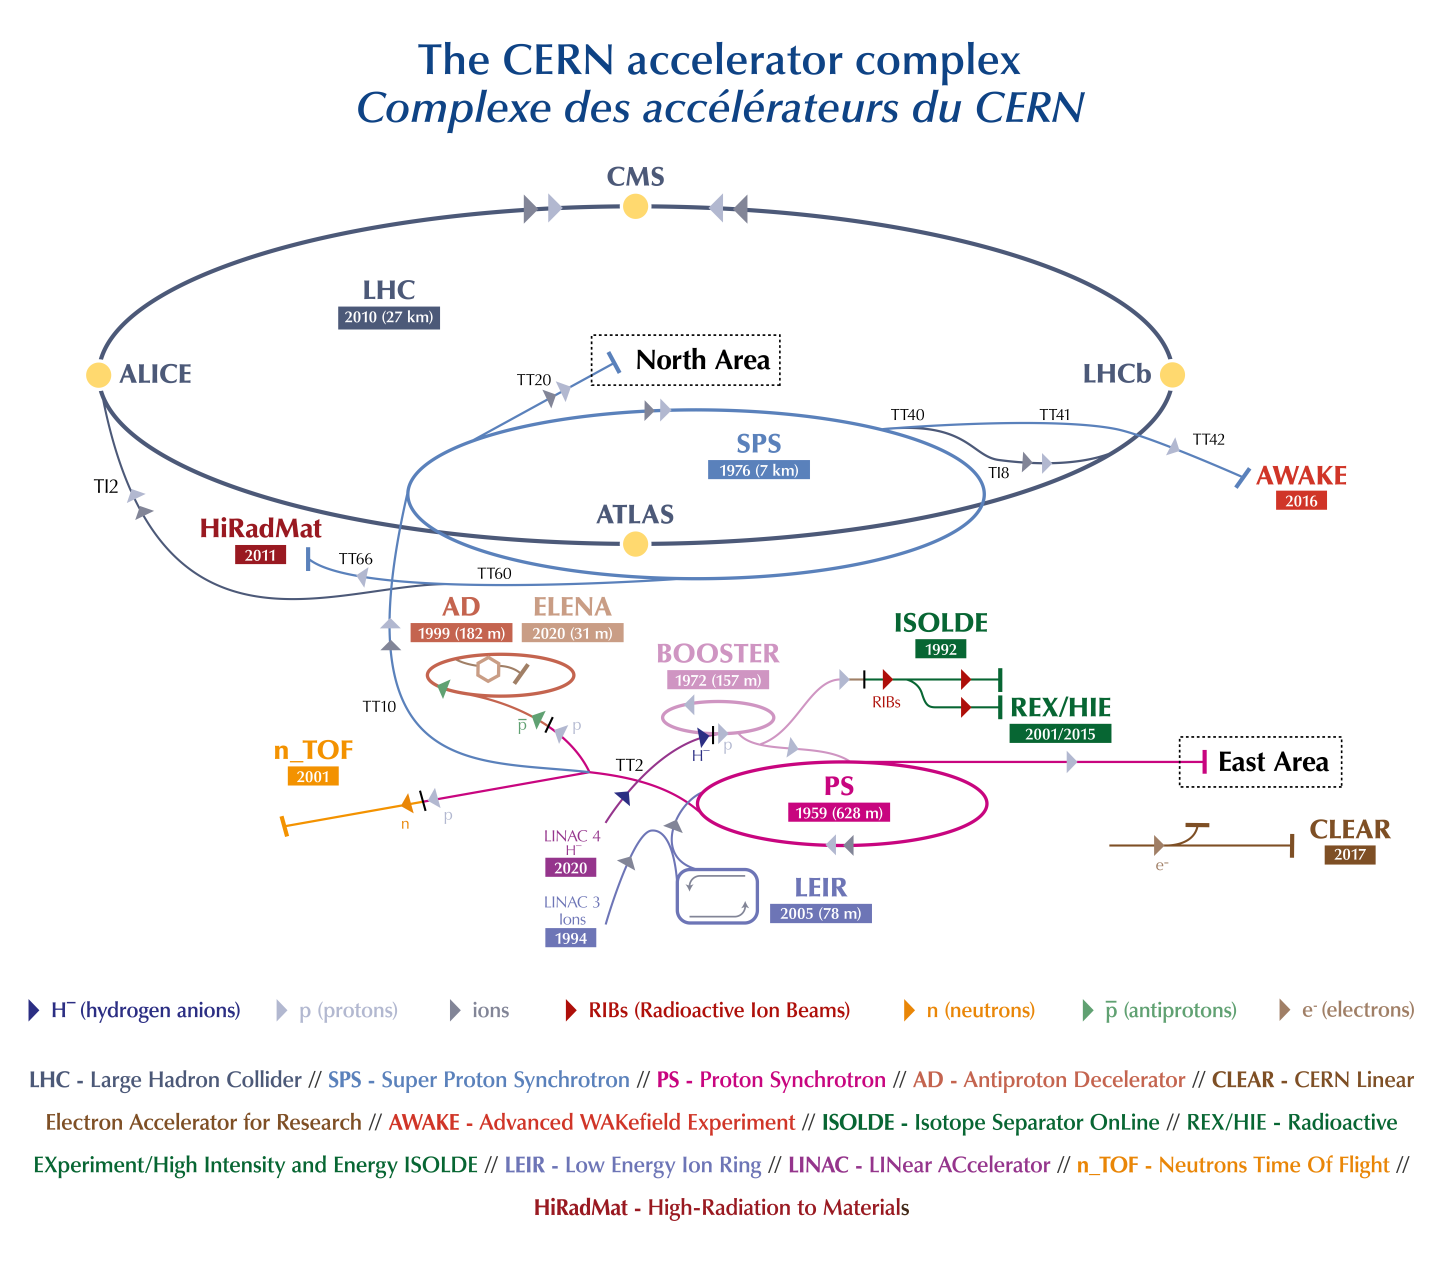
\includegraphics{cern_acc_complex.png}
    \caption{Übersicht des Beschleunigerkomplexes (Quelle: CERN)}
    \label{fig:cern_acc_complex}
\end{figure}

\subsection*{Zielsetzung meines Praktikums}

Ich arbeitete an der der Quelle des Linac3, einer Electron Cyclontron Resonance (ECR) Quelle, die zur Erzeugung von hoch geladenen Schwerionen (hauptächlich Blei) genutzt wird. An dieser Stelle möchte ich nicht auf die Wirkungsweise eingehen, sondern auf \cite{Brown:IonSources} verweisen, da meine Tätigkeit wenig mit der Physik zu tun hatte. Das Ziel, für welches ich eingestellt wurde, war es, verschiedene Machine Learning Ansätze zu erarbeiten, mit denen der Betrieb der Quelle unterstützt werden könnte.

\begin{figure}
    \centering
    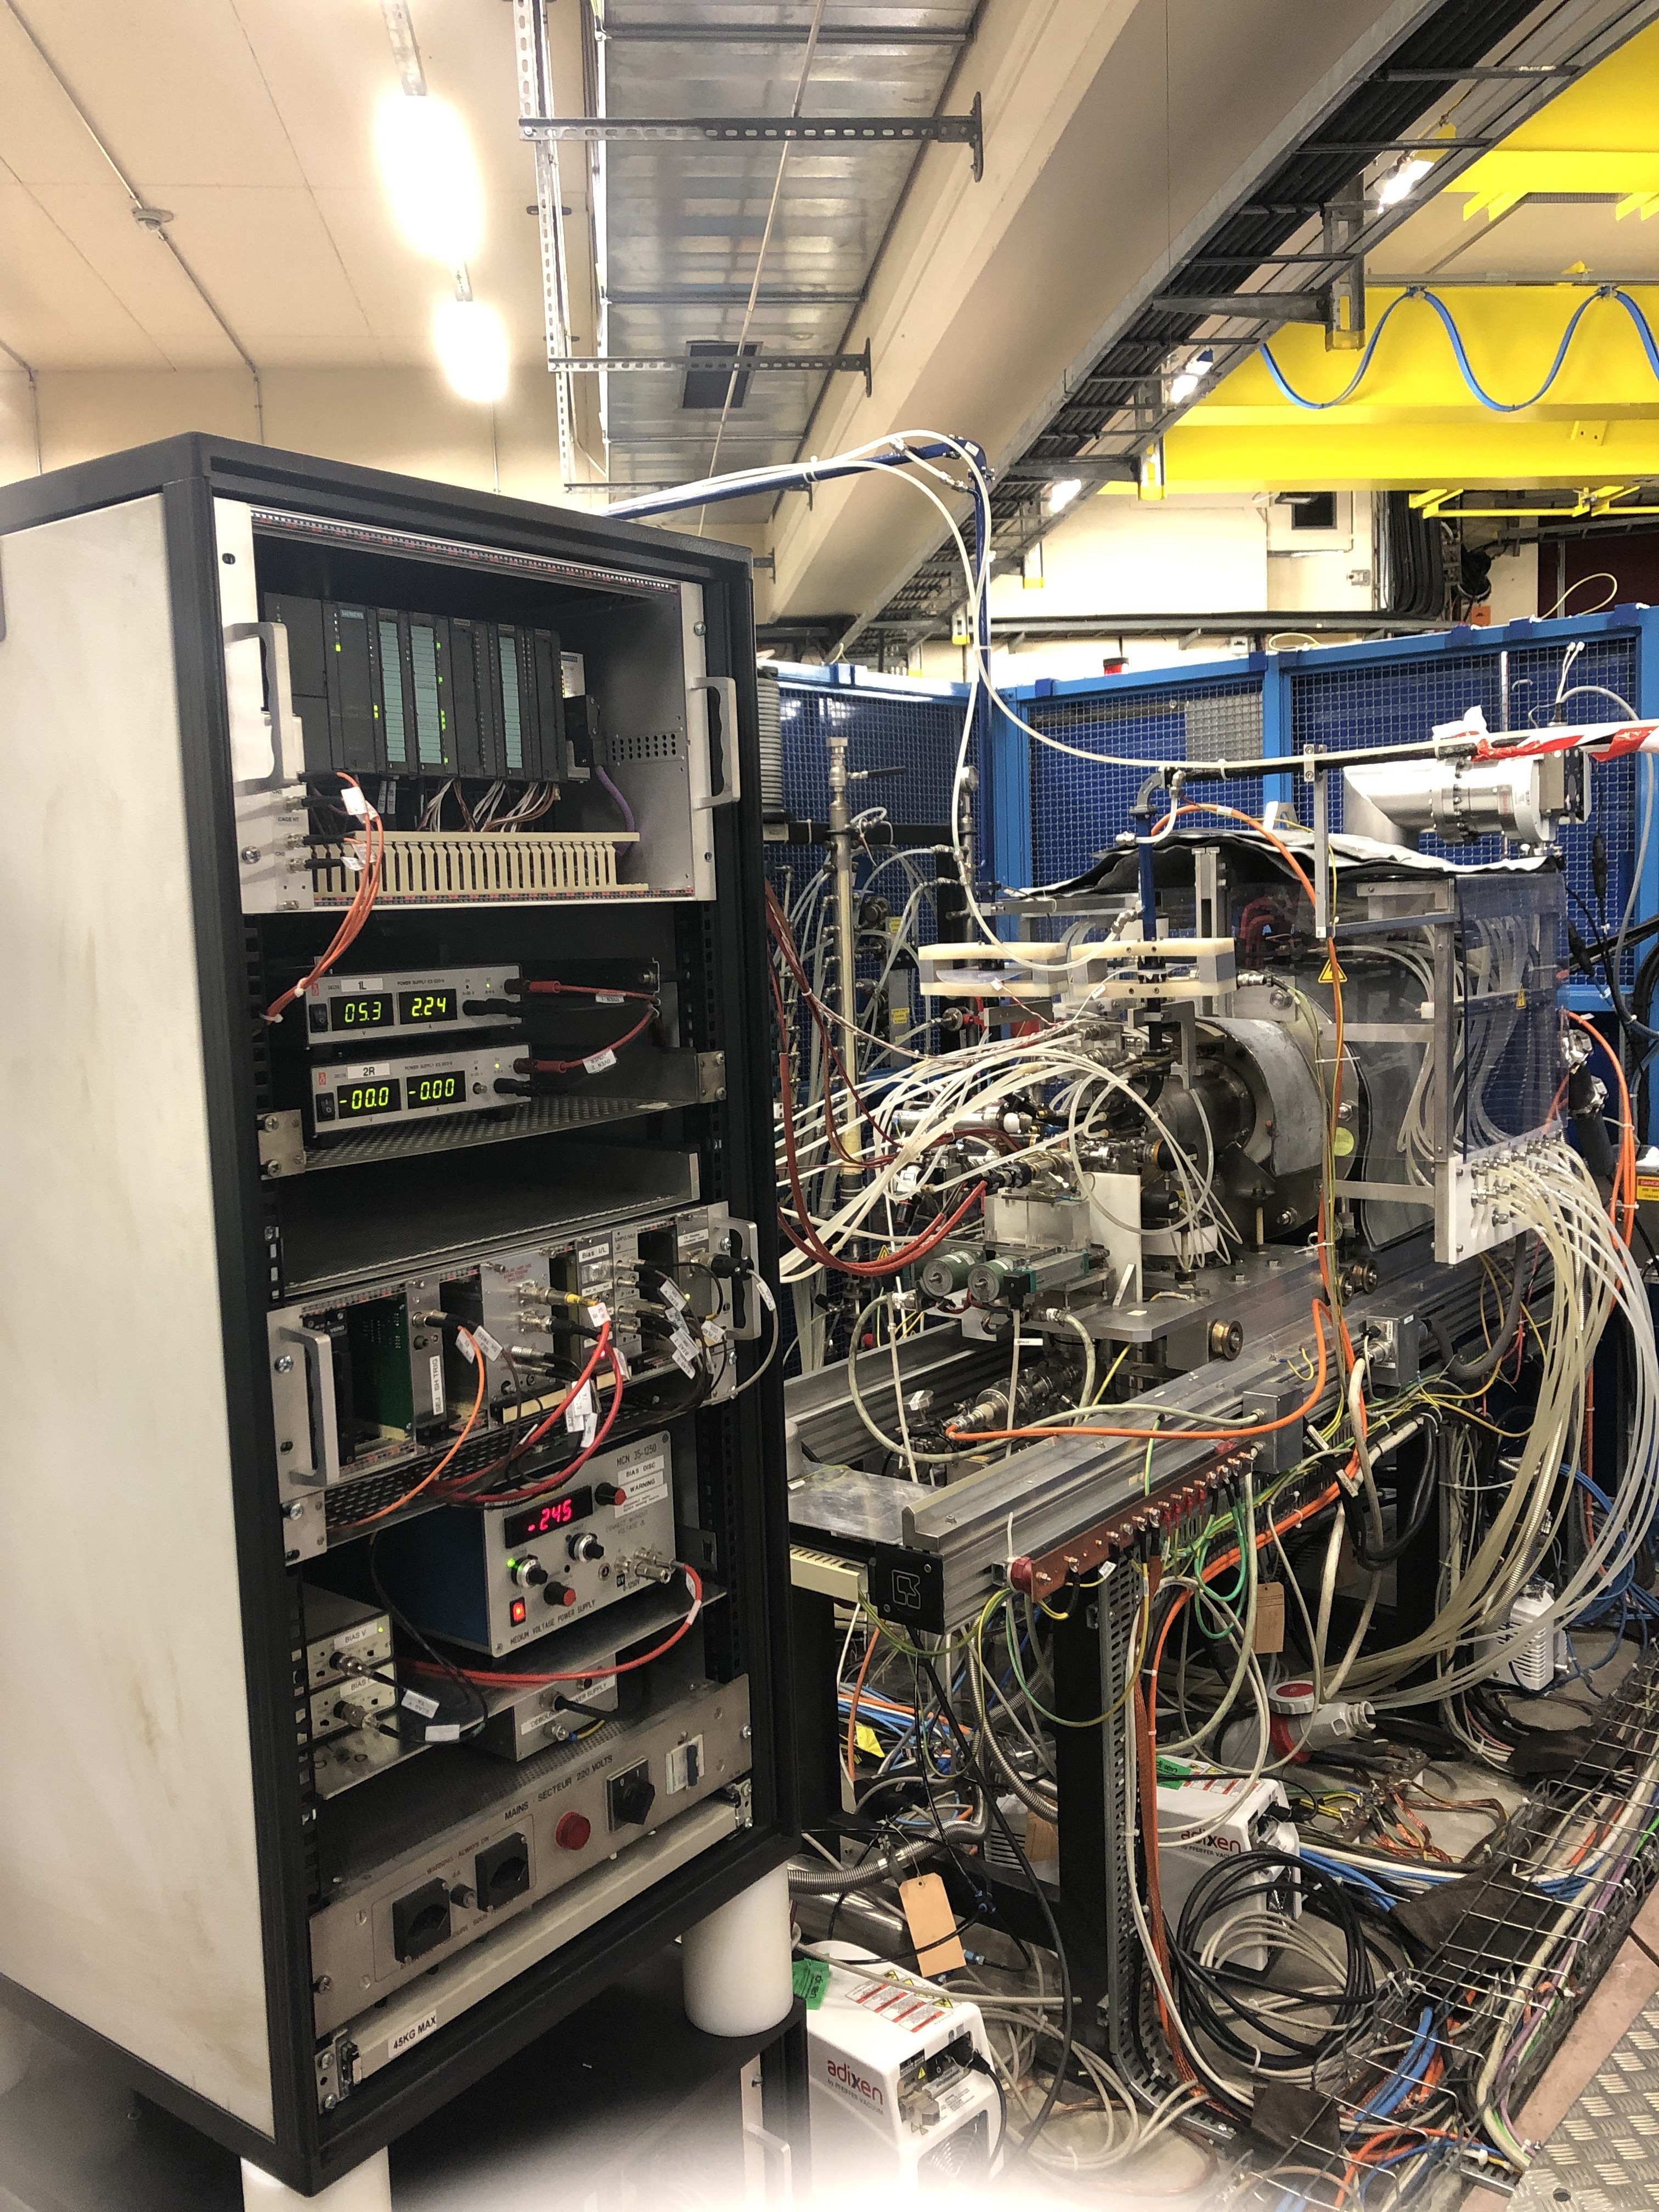
\includegraphics[width=1\textwidth]{gts.jpg}
    \caption{Bild der Linac3 ECR Quelle zur Produktion von Schwerionen. Im Vordergrund zwei Regler für die Stromversorgung sowie Regler für die Spannung an der Bias Disc. Im Hintergrund die eigentliche Quelle mit den zwei mobilen Öfen die mit Blei befüllt werden (Metallröhren an denen dicke, rote Kabel hängen). }
    \label{fig:gts}
\end{figure}

Während der Operation, insbesondere in der Phase wenn die Experimente Strahl beziehen, ist es wichtig, einen intensiven und stabilen Strahl zu liefern. Eine möglichst hohe Intensität ist wichtig, um die Wahrscheinlichkeit von Kollisionen durch eine höhere Zahl von Teilchen zu erhöhen, und eine hohe Stabilität ist wiederum wichtig, damit der Strahl möglichst homogen ist. Ein Auszug der Intensität ist beispielhaft in Abbildung \ref{fig:current_demo} zu sehen.

\begin{figure}
    \centering
    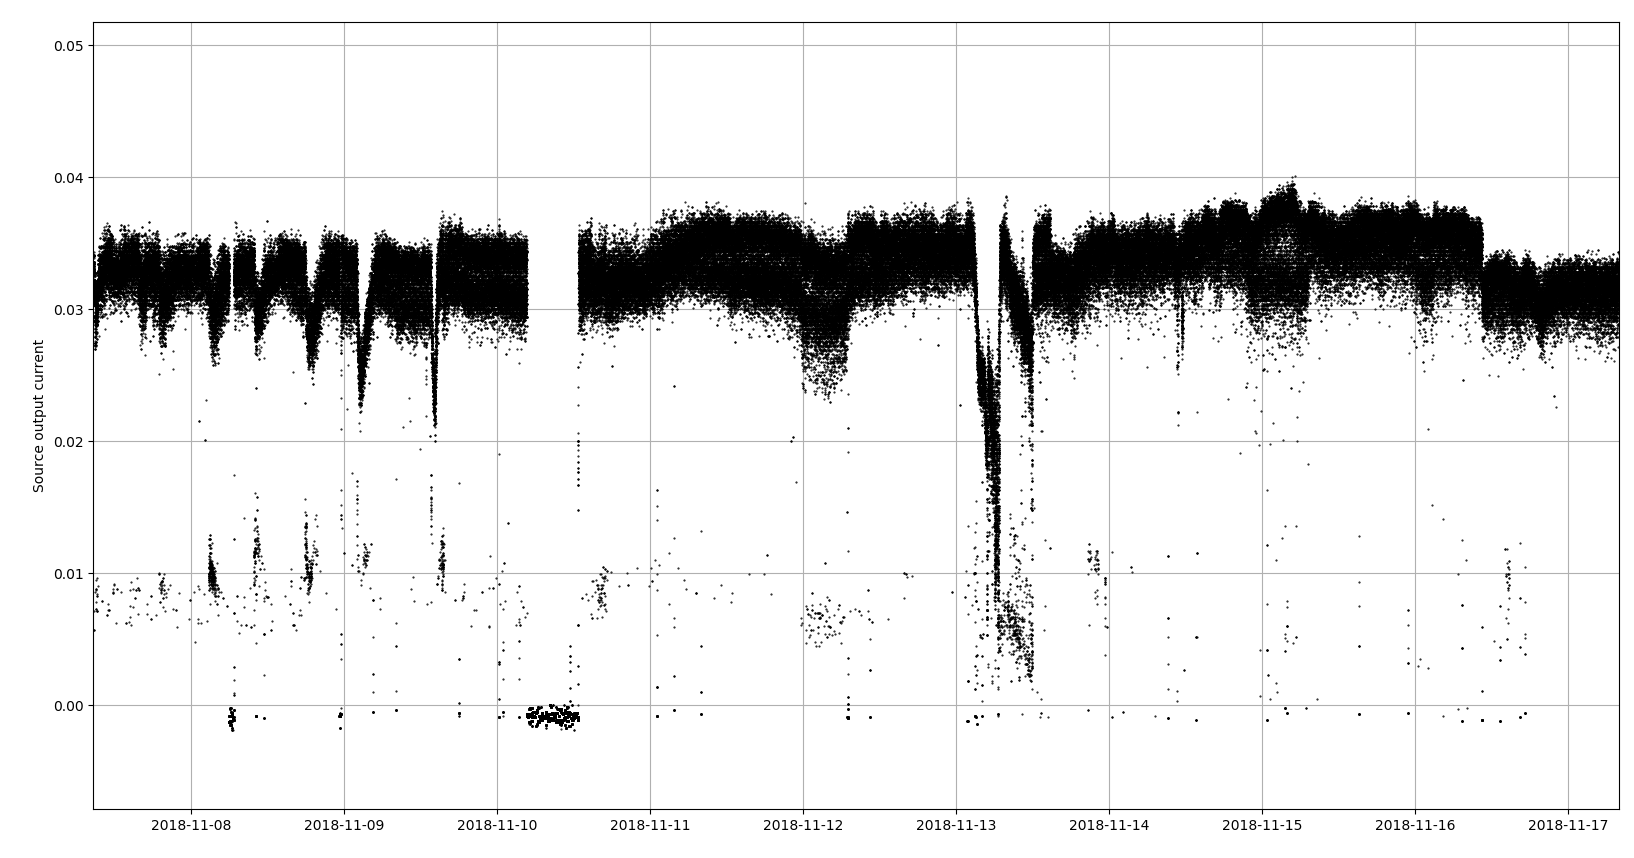
\includegraphics[width=0.9\textwidth]{current_demo.png}
    \caption{Intensität des Strahls in mA, gemessen im Linac3. Periode von 9 Tagen im Physikrun im November 2018. Zu dieser Zeit wird Strahl in den LHC geschickt für Pb-Pb Kollisionen, weshalb eine hohe Intensität und Stabilität entscheidend sind.}
    \label{fig:current_demo}
\end{figure}

Um dieses Ziel zu erreichen, muss die Quelle im laufenden Betrieb manuell nachjustiert werden, in dem verschiedene Einstellungen laufend angepasst werden. Diese Einstellungen sind beispielsweise die Leistung der Verdampfungsöfen oder die Stärke des Magnetfeldes, welches in der Plasmakammer herrscht, und insgesamt gibt es acht Parameter, die verändert werden können. Dieser Nachjustierungsprozess wird von einigen wenigen Quellenexperten durchgeführt, die damit Erfahrung gesammelt haben. Seit einiger Zeit besteht der Wunsch, dies durch Automatisierung zu unterstützen, so wie es beispielsweise an der $H^-$ Quelle des Linac4 getan wird, wo eine Feedbackloop den Strahl vollautomatisiert über lange Perioden stabil halten kann \cite{Voulgarakis:Autopilot}. In meinem Praktikum beschäftigte ich mich hauptsächlich damit, diese Automatisierung voranzutreiben und mögliche Wege zu erforschen, wie Machine Learning dafür verwendet werden könnte.

\section{Meine Aufgaben}

Während meiner Zeit arbeitete ich an einigen Projekten, die ich im Folgenden näher ausführen werde. Ich werde dabei die Ziele eines jeden Projekts beschreiben und erläutern, wie ich vorging, um diese zu erreichen. Mein Betreuer am CERN war einer der oben erwähnten Quellenexperten und der Hauptverantwortliche für das Tuning. Dementsprechend standen wir in einem sehr regen Austausch und er benutzte meine Analysen, um Schlüsse für die Operation zu ziehen.

\subsection*{Clusteranalyse}

Mein Hauptprojekt, mit welchem ich mich das erste halbe Jahr beschäftigte, war die Durchführung einer Analyse der verwendeten Quelleneinstellungen in den Jahren 2015, 2016 und 2018. An diesem Projekt arbeitete ich selbständig, und mein Betreuer validierte die Resultate und formulierte die Fragen, welche für ihn von Interesse waren. Diese Jahre wurden ausgewählt, da in diesen Jahren Bleiionen erzeugt wurden, und für meinen Betreuer das Verstehen der Quelle im Bleimodus aufgrund der Komplexität von vorrangigem Interesse war.

Das Ziel der Analyse war es, einige offenen Fragen zu klären, die den Operatoren helfen sollten, besser zu verstehen wie die Quelle betrieben wurde. Dazu gehörten unter anderem die folgenden Fragen: 

\begin{itemize}
    \setlength\itemsep{-0.2cm}
    \item Gibt es Sätze von Einstellungen, die immer wieder verwendet werden?
    \item Führen bestimmte Einstellungen zu einem tendenziell stabilen oder instabilen Strahl?
    \item Gibt es einen Zusammenhang zwischen Einbrüchen der Hochspannung (dies ist ein scheinbar zufälliger Prozess, der die Quelle für einige Minuten außer Betrieb setzt) und den verwendeten Einstellungen?
\end{itemize}

Um diese Fragen zu beantworten, sollte ein Cluster Algorithmus verwendet werden, um Häufungen von Datenpunkten im Raum der Einstellungen zu finden. Außerdem mussten Phasen des Strahl als stabil bzw. instabil klassifiziert werden. Dies erreichte ich, indem ich in kurzen Zeitfenstern die Strahlintensität und dessen Schwankung mit vorher definierten Grenzwerten verglich.

Aus dem Studium waren mir bereits verschiedene Cluster Algorithmen bekannt (beispielsweise K-Means und DBSCAN), und ich hatte ein ungefähres Verständnis für mögliche Probleme und Lösungsstrategien. Da es sich beim Clustern um eine unüberwachte Lernmethode handelt, d.h. zu den Inputdaten sind keine Outputklassen bekannt, da diese (die Cluster) vom Algorithmus bestimmt werden sollen. Dementsprechend können verschiedene Algorithmen sehr unterschiedliche Resultate liefern, und der Anwender muss diese auf ihre Plausibilität hin überprüfen.

Dementsprechend verbrachte ich sehr viel Zeit damit, ein Gefühl für die Rohdaten zu gewinnen, indem ich die Plotting-Tools der Operatoren verwendete (alle Einstellungen sind über Jahre in einer zentralen Datenbank gespeichert und können mit einem Programm namens \textit{Timber} extrahiert und visualisiert werden), und indem ich eigene Python Skripte schrieb um beispielsweise die Verteilungen der Einstellungen zu verstehen. Dieser Prozess zog sich über mein gesamtes Praktikum, da ich mit immer neuen Sichtweisen neue Zusammenhänge sah, und schloss auch meinen Betreuer stark ein, der mir häufig die physikalischen oder operationellen Hintergründe erläutern konnte.

Des Weiteren investierte ich Zeit in theoretische Recherche, um weitere Algorithmen zu finden, die auf unsere Problemstellung zugeschnitten waren. Beispielsweise handelte es sich in unserem Fall um mehrere Millionen Datenpunkte in bis zu zehn Dimensionen, weshalb Performanz und insbesondere auch der Umgang mit der hohen Dimensionalität relevant waren (siehe beispielsweise \cite{Verleysen:CurseDimensionalityData} für einen Überblick über den Fluch der Dimensionalität).

Anschließend musste eine Infrastruktur erstellt werden, um die Daten auswerten zu können. Hierfür verwendete ich Python in Kombination mit \textit{matplotlib} und Bibliotheken wie \textit{scikit-learn} und \textit{numpy}, um vom Download der Daten, zur Implementierung der Algorithmen, hin zum Plotting der relevanten Graphen und Informationen alles zu bündeln, damit es möglichst einfach auch für zukünftige Analysen verwende werden könne, was auch das Schreiben von ausführlicher Dokumentation einschloss. Der Code zu diesem Projekt befindet sich auf github \cite{Mihailescu:ionsrcopt}.

Aufgrund meiner fehlenden Erfahrung mit der Quelle im laufenden Betrieb, stellte sich schnell ein iterativer Arbeitsprozess in enger Zusammenarbeit mit meinem Betreuer ein, mit dem ich mich mindestens ein mal wöchentlich -- meistens mehrmals -- traf, um die Zwischenergebnisse auszuwerten. Das Feedback konnte ich anschließend benutzen, um meine Analyse weiter zu verfeinern. Ein Beispiel dafür ist, die oben angesprochene Notwendigkeit, die Resultate des Clusteringalgorithmus zu überprüfen. Die Quelle reagiert sehr sensibel auf Änderungen der Einstellungen, so kann beispielsweise eine kleine Veränderung der Ofenleistung bereits große Auswirkungen haben. Dementsprechend hatten wir für die gefundenen Cluster die Anforderung, dass jedes Cluster nur eine ganz kleine Schwankung in der Ofenleistung aufzeigen soll. Mein Betreuer bewertete die Qualität und ich konnte daraufhin die Parameter des Algorithmus besser anpassen.

Schlussendlich konnten wir die Ergebnisse in einem Bericht zusammenfassen und unserer Abteilung präsentieren. Ernüchternderweise produzierte die Analyse allerdings negativ Resultate, beispielsweise konnten wir nicht belegen, dass bestimmte Einstellungen einen stabilen Strahl produzieren. Dennoch konnten wir zeigen, dass das ursprüngliche Ziel der Automatisierung komplizierter zu erreichen war als angenommen, und konnten Impulse setzen, in die weiter recherchiert werden sollte. Dennoch war das Ausbleiben eines Erfolges für mich persönlich ein kleiner Rückschlag und ich musste lernen damit umzugehen, dass es nicht zu jedem Problem eine offensichtliche Lösung gibt.

\subsection*{Change Point Analyse}

Nachdem wir festgestellt hatten, dass eine automatische Regulierung der Einstellungen zum damaligen Zeitpunkt nicht möglich war, kamen wir zu dem Schluss, dass ein Frühwarnsystem für die Operation sehr hilfreich wäre. In Abbildung \ref{fig:current_demo} sieht man, dass der Strahl immer wieder an Intensität verliert oder die Varianz steigt. Beides sind Effekte die vermieden werden sollten, und ein sehr frühes Erkennen solcher Instabilitäten könnten ein schnelles manuelles Eingreifen ermöglichen um diesen Entgegenzusteuern.

Wenn sich Chrakteristische Merkmale einer Zeitreihe ändern, bezeichnet man dies in der Literatur als \textit{Changepoint} \cite{Aminikhanghahi:surveymethodstime}. Ich beschäftigte mich damit, verschiedene Algorithmen die für das Detektieren dieser Changepoints existieren auf die Linac3 Quelle anzuwenden.

Mein Fokus lag dabei auf dem Erkennen von Veränderungen von Strahlcharakteristiken, insbesondere im Erkennen von plötzlichen Intensitätsveränderungen und dem Auftreten starker Schwankungen. Ziel hierfür war es, eine Methode zu finden, die auch im laufenden Betrieb funktionierte, d.h. es gab die Anforderung online zu arbeiten. Dafür erwies sich ein bayes'scher Ansatz als hilfreich, beschrieben in \cite{Adams:BayesianOnlineChangepoint}. Dieser Algorithmus schätzt sogenannte \textit{Runlength Wahrscheinlichekeiten}, die Wahrscheinlichkeit, dass ein Changepoint $x$ Zeiteinheiten vom aktuellen Moment zurückliegt.

Neben der Implementierung beschäftigte ich mich damit, effektive Hyperparameter für den Algorithmus zu finden und nach Möglichkeiten zu suchen, die Ergebnisse zu optimieren und stabiler zu machen. Dafür recherchierte ich auf dem ursprünglichen Artikel basierende Konzepte und experimentierte mit eigenen Optimierungen des Algorithmus. 

Auf Grund von Zeitmangel konnte diese Projekt leider nicht zur Anwendungreife fertiggestellt werden, aber ich bin optimistisch, dass dieses Gerüst in Zukunft weiterentwickelt werden kann, um die Operation als Frühwarnsystem zu unterstützen. In Abbildung \ref{fig:bocd} sieht man eine beispielhafte Anwendung, die schwarzen Balken zeigen einen vom Algorithmus gefundenen Changepoint. Außerdem präsentierte ich den Ansatz in einem informellen Machine Learning Forum, wo er Anklang fand und dadruch hoffentlich auch von anderen Teams einbezogen wird.

\begin{figure}
    \centering
    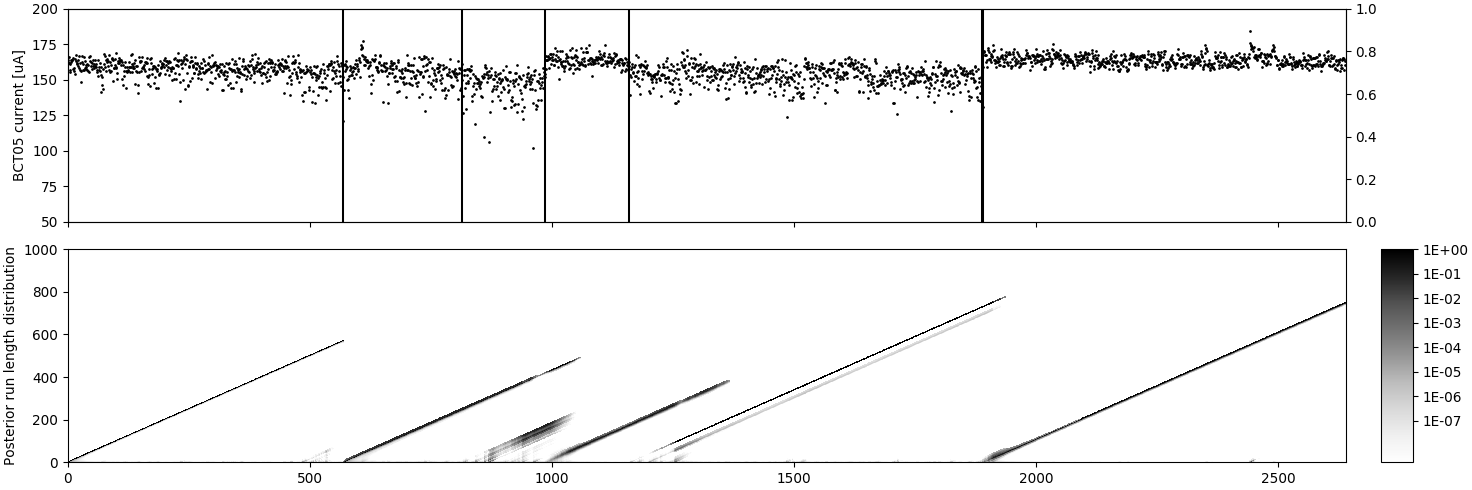
\includegraphics[width=0.9\textwidth]{bocd_example.png}
    \caption{Der BOCPD Algorithmus angewandt auf ungefähr sieben Stunden Strahl (Bleiionen gemessen am Ausgang der Quelle) aus September 2018. Schwarze Balken im oberen Plot zeigen vom Algorithmus gefundene Changepoints. Im unteren Plot ist die (log-) Wahrscheinlichkeit für verschiedene Runlenghts abgebildet. Dunklere Pixel repräsentieren eine höhere Wahrscheinlichkeit.}
    \label{fig:bocd}
\end{figure}

\subsection*{Autopilot}

Ein weiteres, mehr angewandtes Projekt mit dem ich beauftragt wurde, war die Adaption eines Autopilotsystems für den Linac3. Für den Linac4 gibt es wie weiter oben erwähnt verschiedene Feedbackschleifen, die einen (halb-)automatischen Betrieb ermöglichen. Diese Schleifen werden von einem zentralen Server gesteuert, auf welchem verschiedene Pythonskripte laufen, die mit den Maschinen rückkoppeln. Dieses System wurde während meines Praktikums auch für den Linac3 installiert, und ich kümmerte mich um die Adaption bereits existierender Tools, sowie um Tests der Funktionen.

Die Skripte, die auf dem Server laufen, nennen sich entweder \textit{Monitors} oder \textit{Actors}. Monitore bündeln Daten von verschiedenen Messstationen und veröffentlichen sie dann als ein Paket, welches von Actors empfangen werden kann, um daraufhin Maschinen zu steuern. 

Meine Aufgaben war es, solche Monitore und Actors zu schreiben, um die Hochspannung in der Quelle (eine der Einstellungsmöglichkeiten) anzupassen, um die Strahlintensität zu maximieren. Dazu musste ich eine bereits existierende Logik auf das neue System anpassen, d.h. das neue Pythonframework auf unseren Anwendungsfall adaptieren. Diese Skripte werden genauso wie reelle Maschinen zentral verwaltet, weshalb sie auch teils auch als virtuelle Maschinen bezeichnet werden. Diese müssen in den zentralen Datenbanken eingetragen werden, damit das System weiß, welche Parameter gespeichert werden und was als Output erwartet wird. Auch dieses Management war meine Aufgabe im Autopilot-Projekt.

Da ich damit der erste Benutzer dieser Infrastruktur war, vertrauten die Verantwortlichen auf mein Feedback bezüglich Stabilität und Nutzerfreundlichkeit des Systems, da ich stetig auswertete, ob die korrekten Daten übertragen wurden. Dadurch konnten wir verschiedene Serverausfälle diagnostizieren und deren Ursachen beheben.

Durch meine Intensive Einarbeitung in die Plattform diente ich auch als Ansprechpartner für das System innerhalb der Abteilung und half zwei Kollegen ihre Skripte für die Maschine auf das neue System zu portieren.

\subsection*{Weiteres}

Zusätzlich zu den großen Projekten hatte ich noch eine Reihe an kleineren Aufgaben.

In einer anderen Abteilung von Beams gab es ebenfalls ein kleines Team, dass sich mit maschinellen Lernen für den Linac3 beschäftigte. Im Unterschied zu unserer Analyse, die darauf ausgerichtet war besser zu verstehen, wie die Operatoren die Quelle justieren, verfolgte dieses einen Ansatz mit neuronalen Netzwerken zur Vorhersage von Charakteristiken des Strahls, beispielsweise der Intensität. Ich koordinierte regelmäßige Treffen und präsentierte mehrmals unsere Fortschritte, um so einen Wissensaustausch zu ermöglichen. Zusammen mit meinem Betreuer konnte ich durch die Erfahrung die ich durch die Datenanalyse sammelte Vorschläge liefern, welche Größen als Vorhersageziel und welche Parameter als Inputs sinnvoll wären.

Des Weiteren fanden alle zwei Wochen (zumindest vor Beginn der Covid-19-Pandemie, später seltener), abteilungsinterne Meetings, die \textit{Ion-Source-Meetings}, statt, die als Plattform für technischen Austausch über neue Ergebnisse dienten. Ich war zuständig dafür, diese mit zu organisieren und musste beispielsweise die Events auf einer Onlineplattform erstellen und Einladungen verschicken.

Außerdem verbrachte ich einiges an Zeit mit Recherche und Experimentieren mit verschiedenen anderen Machine Learning Methoden für die Quelle, die ich nicht einem Projekt zuordnen kann. Dazu musste ich einige Algorithmen in Python implementieren und mir Wege überlegen, sie auf unsere Daten anzuwenden. Diese Recherche dient als Grundlage für weitere Möglichkeiten der Automatisierung und wird hoffentlich von einem möglichen Nachfolger verwendet werden. Einen Bericht den ich darüber geschrieben habe findet man in \cite{Mihailescu:MLresearch}.

\section{Fazit}

Meine Erwartungen an das Praktikum wurden zum großen Teil erfüllt. Insbesondere die wissenschaftliche Atmosphäre hat mir sehr gut gefallen und mich motiviert, viel zu lernen. Dadurch, dass die Zielsetzungen weniger ergebnisorientiert waren, als es in einem Unternehmen vermutlich der Fall gewesen wäre, hatte ich viel Freiraum, mich tiefgreifend mit der Materie zu beschäftigen und eigenen Ideen nachzugehen und diese umzusetzen. Von den Kollegen wurde ich darin stets bestärkt und ich habe mich dadurch in meinem Team sehr wertgeschätzt gefühlt. Des Weiteren hatte ich die Möglichkeit eine Reihe an Menschen kennenzulernen, die in anderen Bereichen arbeiteten, und konnte so auch einen Einblick darin bekommen, welche weitere Anwendungsgebiete Machine Learning in der Hochenergiephysik besitzt.

Die Aufgaben, um die ich mich gekümmert haben, waren ebenfalls sehr spannend für mich. Durch meine sehr selbstständige Arbeitsweise habe ich neben fachlicher Expertise auch sehr viel über Projekt- und Softwaremanagement gelernt, sowie durch regelmäßige Präsentationen auch über das Präsentieren für verschiedenes Publikum. Dadurch, dass ich viele wissenschaftliche Publikationen aus der Informatik und Datenverarbeitung las, hatte ich das gesamte Praktikum über einen sehr großen Studiumsbezug, und konnte die methodische und strukturierte Denkweise täglich anwenden.

Leider hatte ich in meiner Abteilung als einziger einen mathematisch-informatischen Hintergrund, weshalb ich teilweise etwas alleine vor Problemen stand. Ich denke ich hätte davon profitiert, mich mit jemandem über die Fragestellungen auszutauschen, der ebenfalls eine auf Algorithmen ausgerichtete Sichtweise eingenommen hätte, da ich der Meinung bin, dass dadurch andere Impulse ausgelöst werden wären.

Erschwert wurde mein Praktikum leider auch durch die Covid-19-Pandemie, wegen der das CERN für mehrere Monate auf minimale, absolut notwendige Präsenz reduziert wurde, und wegen der ich knapp vier Monate im Homeoffice arbeitete. Dadurch wurde es schwieriger, Arbeit aus anderen Bereich mit zu bekommen, und man fokussierte sich meiner Meinung nach leider zu sehr auf seine eigenen Aufgaben. Trotzdem war die Kommunikation mit den für mich relevanten Kollegen unproblematisch und da meine Aufgaben keine Präsenz erforderten, fühlte ich mich dadurch kaum eingeschränkt.

Dennoch blicke ich sehr positiv auf mein Praktikum zurück. Ich habe sehr viel daraus mitgenommen und gemerkt, dass mir ein Beruf mit Forschungsfreiheiten -- sei es in einem Unternehmen oder einer anderen Organisation -- bei dem es um Datenanalyse geht, zusagt. Hier werde ich in Zukunft Wert darauf legen, die Möglichkeit für Ideenaustausch zu haben. Auch die Selbstständigkeit die ich genossen habe war mir sehr wichtig. Zusammenfassend kann ich sagen, dass mir das Praktikum sehr bei der zukünftigen Berufswahl geholfen hat, und ich die Auszeit vom Studium gut nutzen konnte, um mich persönlich weiterzuentwickeln.

\clearpage
\printbibliography
\end{document}